\subsection{Definici\'on}

Hans Schmid propuso una definici\'on para los materiales multiferroicos en la cual se denomina de esta manera a todos aquellos materiales que presentan una coexistencia de dos o m\'as ordenes ferroicos primarios en la misma fase cristalina. Dichos ordenes ferroicos primarios son : ferroelasticidad, ferromagnetismo y actualmente tambi\'en se ha propuesto considerar la ferrotoroicidad \cite{esrenstein2006}.


\noindent La posibilidad de controlar las propiedades f\'isicas macrosc\'opicas es una caracter\'istica com\'un de los materiales multiferroicos. Por ejemplo, la magnetizaci\'on o la deformaci\'on en el caso de los ferroel\'asticos puede ser cambiada aplicando un campo el\'ectrico o magn\'etico al material incluso es posible conseguir este efecto por medio de una deformaci\'on mec\'anica. Como se mencion\'o la ferrotoroicidad es estudiada como un orden ferroico primario. Esta propiedad es presentada por los materiales cuyo momento magn\'etico es generado por una orientaci\'on circular. Estos momentos magn\'eticos toroidales presentan acoplamiento magnetoel\'ectrico, dicha propiedad genera inter\'es debido a que la aplicaci\'on de un campo magn\'etico sobre un toroide influye en la polarizaci\'on \cite{nazzen1988}.


%===================================================
\subsection{Propiedades}
% #######################################
\subsubsection{Ferroelectricidad}

Cuando un material presenta un momento dipolar el\'ectrico en ausencia de un campo el\'ectrico externo se le denomina ferroel\'ectrico. Esto es debido a que los centros de las cargas positivas y negativas no coinciden en la estructura cristalina. Existe una temperatura limite por debajo de la cual un material puede presentar ferroelectricidad, dicho limite se conoce como la temperatura de Curie, que al ser sobrepasada provoca que el material pase a un estado parael\'ectrico. Este estado parael\'ectrico se asocia con un decaimiento r\'apido de la constante diel\'ectrica \cite{kimura2003}.

\noindent La facilidad para crear dipolos orientados en la direcci\'on de un campo externo define la polarizabilidad de un material \cite{smith1993}. La suma de los momentos dipolares da origen al vector de polarizaci\'on {\bf P} por lo que en ausencia de un campo externo, {\bf P} es cero desde un punto de vista macrosc\'opico. Esto se da incluso si las mol\'eculas tienen un momento dipolar diferente de cero, dado que estos se anulan dentro de la estructura cristalina. Al ser aplicado un campo el\'ectrico externo la polarizaci\'on aumenta debido a lo siguiente:

\begin{itemize}
    \item Si existen dipolos permanentes, estos se reorientan definiendo una polarizaci\'on dipolar.
    \item La polarizaci\'on i\'onica generada por los movimientos de los iones tambi\'en contribuye.
    \item El desplazamiento de las nubes de electrones considerando una red inm\'ovil de iones que da origen a la polarizabilidad electr\'onica tambi\'en contribuye.
\end{itemize}

\noindent La permitividad $\varepsilon$ o la susceptibilidad $\chi$ definen la polarizabilidad del material.

\begin{equation}
P = \varepsilon _{0} \chi E
\label{polarizacion} \textrm{ ,}
\end{equation}

\begin{equation}
\varepsilon = \varepsilon _{0}E+P
\label{permitividad} \textrm{ ,}
\end{equation}

\noindent donde $\varepsilon _{0}$ es la permitividad el\'ectrica del vac\'io.

\noindent Una caracter\'istica de los ferroel\'ectricos es presentar un momento dipolar diferente de cero por celda unitaria el cual se asocia con valores elevados de $\varepsilon$. No es posible que un material ferroel\'ectrico sea cubico debido a que dicha simetr\'ia cancelar\'ia los momentos dipolares.

%##########################################
\subsubsection{Ferromagnetismo}

El ferromagnetismo se presenta en compuestos met\'alicos. Estos materiales presentan un momento magn\'etico permanente incluso en ausencia de un campo externo. Adem\'as, estos materiales presentan valores de magnetizaci\'on altos que pueden ser permanentes considerando peque\~nos dominios. Estas caracter\'isticas se presentan en metales de transici\'on como el hierro, cobalto o niquel y en tierras raras como el gadiolinio \cite{kimura2003}.

\noindent Los materiales ferromagn\'eticos poseen dominios magn\'eticos por debajo de la temperatura de Curie ($T_{c}$). Estos dominios magn\'eticos son peque\~nas regiones donde existe magnetizaci\'on espont\'anea cuya orientaci\'on es al azar en ausencia de un campo magn\'etico externo, de esta forma los efectos magn\'eticos se cancelan desde un punto de vista macrosc\'opico. Al aplicarse un campo magn\'etico externo los dominios se reorientan en la direcci\'on del campo y aumentan su tama\~no. Al ser retirado el campo externo los dominios regresan a su estado inicial dando origen al fen\'omeno de hist\'eresis \cite{kimura2003}.

\noindent La relaci\'on entre la susceptibilidad magn\'etica y la
temperatura en los materiales ferromagn\'eticos esta dada por la ley de Curie-Weiss (ec. \ref{curie_weiss}) que modifica la ley de Curie (ec. \ref{curie}).


\begin{equation}
\chi = \frac{C}{T}
\label{curie} \textrm{ ,}
\end{equation}

\begin{equation}
\chi = \frac{C}{T-\theta _{p}}
\label{curie_weiss} \textrm{ ,}
\end{equation}

\noindent donde $\theta _{p} = T_{c}$ siempre toma valores positivos en la 
escala absoluta de temperatura. Adem\'as se pueden hallar susceptibilidades magn\'eticas de $10^{6}$ en los materiales ferromagn\'eticos.

%#########################################
\subsubsection{Antiferromagnetismo}

Un material antiferromagn\'etico puede describirse como un conjunto de subredes ferromagn\'eticas antiparalelas entre s\'i que poseen momentos magn\'eticos de igual magnitud. Estas subredes deben ser alternadas para que los momentos magn\'eticos se cancelen entre s\'i. Los materiales antiferromagn\'eticos presenta m\'as de un tipo de ordenamiento, que es clasificado seg\'un la forma en la que est\'an dispuestos los momentos magn\'eticos en la 
red. Se muestran algunos tipos de arreglos antiferromagn\'eticos en la figura \ref{antiferro}.


\begin{figure}[H]
    \centering
    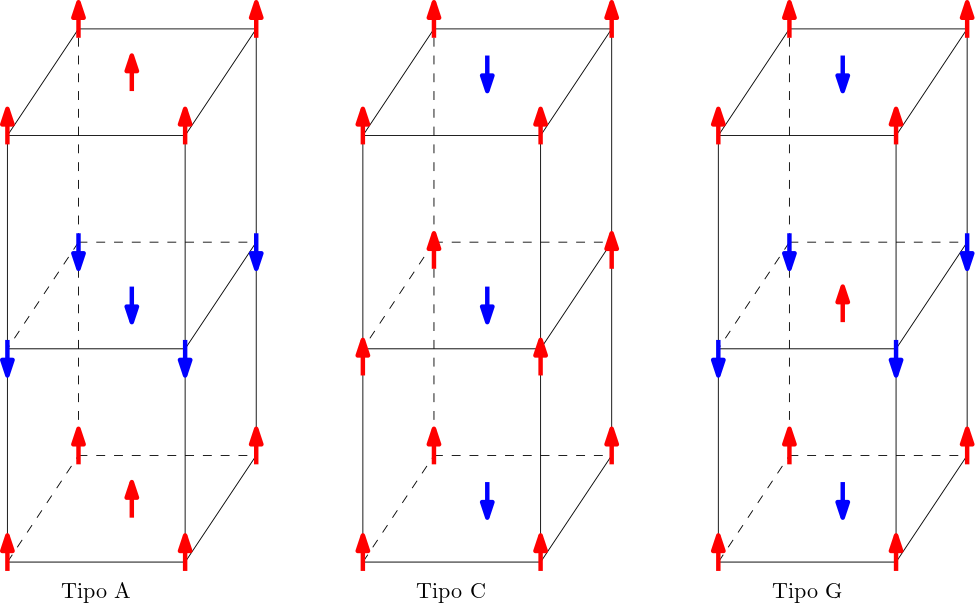
\includegraphics[width=0.6\textwidth]{contenido/marco_teorico/materiales_multiferroicos/img_MaterialesMultiferroicos/tipos_antiferro.png}
    \caption[Tipos de antiferromagnetismo]{Tipos de arreglos 
    antiferromagn\'etico. {\bf Tipo A}: 
        intraplanos ferromagn\'eticos e interplanos antiferromagn\'eticos. {\bf 
        Tipo C}: intraplanos
        antiferromagn\'eticos e interplanos
        ferromagn\'eticos. {\bf Tipo G}: intraplanos antiferromagn\'eticos e 
        interplanos antiferromagn\'eticos.}
    \label{antiferro}
\end{figure}

\noindent La ley de Curie-Weiss (ec. \ref{curie_weiss}) tambi\'en se aplica a los materiales antiferromagn\'eticos donde $\theta _{p}$ toma valores negativos en la escala absoluta de temperatura definiendo la temperatura de N\'eel $T_{N}$.
